\chapter*{}
%\thispagestyle{empty}
%\cleardoublepage

%\thispagestyle{empty}

\begin{titlepage}
 
 
\setlength{\centeroffset}{-0.5\oddsidemargin}
\addtolength{\centeroffset}{0.5\evensidemargin}
\thispagestyle{empty}

\noindent\hspace*{\centeroffset}\begin{minipage}{\textwidth}

\centering
%
\includegraphics[width=0.9\textwidth]{imagenes/logo_ugr.jpg}\\[1.4cm]

%\textsc{ \Large PROYECTO FIN DE CARRERA\\[0.2cm]}
%\textsc{ INGENIERÍA EN INFORMÁTICA}\\[1cm]
% Upper part of the page
% 

 \vspace{3.3cm}

%si el proyecto tiene logo poner aquí
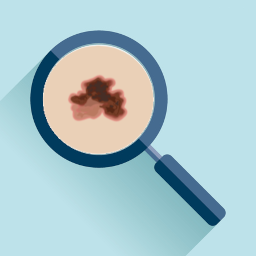
\includegraphics{imagenes/logo.png} 
 \vspace{0.5cm}

% Title

{\Huge\bfseries Aplicación móvil para la prognosis y detección del cáncer de piel usando Deep Learning\\
}
\noindent\rule[-1ex]{\textwidth}{3pt}\\[3.5ex]
%{\large\bfseries Subtítulo del proyecto.\\[4cm]}
\end{minipage}

\vspace{2.5cm}
\noindent\hspace*{\centeroffset}\begin{minipage}{\textwidth}
\centering

\textbf{Autor}\\ {Cristhian Moya Mota}\\[2.5ex]
\textbf{Directores}\\
{Nombre Apellido1 Apellido2 (tutor1)\\
Nombre Apellido1 Apellido2 (tutor2)}\\[2cm]
%
\includegraphics[width=0.15\textwidth]{imagenes/tstc.png}\\[0.1cm]
%\textsc{Departamento de Teoría de la Señal, Telemática y Comunicaciones}\\
%\textsc{---}\\
%Granada, mes de 201
\end{minipage}
%\addtolength{\textwidth}{\centeroffset}
\vspace{\stretch{2}}

 
\end{titlepage}






\cleardoublepage
\thispagestyle{empty}

\begin{center}
{\large\bfseries Aplicación móvil para la prognosis y detección del cáncer de piel usando deep learning}\\
\end{center}
\begin{center}
Cristhian Moya Mota\\
\end{center}

%\vspace{0.7cm}
\noindent{\textbf{Palabras clave}: cáncer de piel, deep learning, prognosis, diagnóstico, preprocesado, cuantización, aplicación Android.}\\

\vspace{0.7cm}
\noindent{\textbf{Resumen}}\\

El cáncer es una de las enfermedades que más muertes causan al año en todo el mundo. Su tendencia, en aumento, refleja la importancia de una correcta detección y diagnóstico de esta enfermedad a través de los médicos especialistas. Sin embargo, su elevado coste en algunos países, y la gran incidencia mostrada cada año dificulta el acceso a los medios adecuados para una parte considerable de la población, sobre todo, aquella con menos recursos. Uno de los más frecuentes, el cáncer de piel, suma a este problema la dificultad de diagnóstico, compleja incluso para los dermatólogos por su similitud con los lunares comunes.

La detección temprana de los tumores cutáneos, sobre todo de los de tipo melanoma, es clave para aumentar la esperanza de vida de sus pacientes. Para hacer más accesible el diagnóstico, se propone el uso de modelos de deep learning, cuyo modelo resultante tras el aprendizaje sea capaz de ejecutarse en un teléfono móvil, teniendo en cuenta las restricciones de potencia asociadas.

Se emplean, para lograrlo, los conjuntos de datos más citados y conocidos del estado del arte, mediante los cuales se procede a la creación de un conjunto combinado variado y suficientemente extenso como para diagnosticar no solo si se trata de una lesión benigna o maligna, si no también para especificar la enfermedad concreta a la que el paciente se enfrenta. Por tanto, convierte el proceso de tratamiento de los datos en un aspecto clave a tener en cuenta, que comprende la selección, el recortado y el reetiquetado manual de los datos para lograr la estandarización de los mismos y obtener un conjunto apto para el proceso de aprendizaje, tras aplicar un aumento de resolución mediante redes generativas adversarias(GANs)~\cite{goodfellow2014generative}.

Para esta tarea, se tienen en cuenta las restricciones de potencia impuestas por la arquitectura ARM de los smartphones, usando para ello el proceso de cuantización de modelos. Tras un análisis de los modelos habitualmente aplicados, se demuestra que la simplificación mediante cuantización consigue mejores resultados que los modelos pensados inicialmente para ser ejecutados en dispositivos de baja potencia. Además, se emplea un enfoque novedoso por el cual, en lugar de construirse un único modelo, se construyen 3 modelos organizados a dos niveles para reducir al mínimo las pérdidas ocasionadas por la cuantización, siendo uno específico para distinguir en un primer nivel, si se trata de una enfermedad maligna o benigna, y posteriormente, emplear uno de los dos modelos especializados en cada una de las variantes.

Esta arquitectura consigue unos resultados cercanos a un 83\% de aciertos en clasificación binaria, y un 82\%  y 45\% en enfermedades malignas y benignas, respectivamente, por lo que ofrece resultados razonables teniendo en cuenta la ganancia en velocidad obtenida tras realizar el proceso de cuantización, superior a 1,5 en los 3 casos. Además, todo ello se consigue con apenas un 1\% de pérdida respecto al modelo base, ResNet50~\cite{he2015deep}

Por último, para poner en práctica el modelo entrenado, se ha desarrollado una aplicación Android que ofrece al usuario la capacidad de tomarse una fotografía de la lesión que desee diagnosticar, y obtener el resultado en un tiempo inferior a un segundo, sin necesidad de conectarse a servidores externos, y con la posibilidad de revisar los casos previamente diagnosticados y su evolución mediante un historial. 

\cleardoublepage
\thispagestyle{empty}


\begin{center}
{\large\bfseries Aplicación móvil para la prognosis y detección del cáncer de piel usando deep learning}\\
\end{center}
\begin{center}
Cristhian Moya Mota\\
\end{center}

%\vspace{0.7cm}
\noindent{\textbf{Keywords}: skin cancer, deep learning, prognosis, preprocessing, quantization,  Android app.}\\

\vspace{0.7cm}
\noindent{\textbf{Abstract}}\\

Cancer is one of the diseases that causes the most deaths each year worldwide. Recent studies say each year there will be more cases than previous. This reflects the importance of preventive detection and diagnosis by specialists . However, preventive medicine has a high cost in some countries. The high incidence shown each year make access to specialists a difficult task for a considerable part of the population, especially those with fewer resources. Skin cancer is one of the most frequent cancers in the world, and its similarity to other skin conditions like benign moles make the problem even harder for specialists.

Preventive medicine is the way to minimize the mortality of some skin cancers, like melanoma, which is the worst posible condition. In order to make prognosis an easier task, we propose the use of deep learning models, with the resulting model after learning being capable of running on a mobile phone, taking into account CPU power restrictions.

To achieve it, this project uses the most used and cited datasets in the state of art. With them, we made a big an exhaustive dataset which combines images to detect if a mole is benign or malign. But, we also have enough information to predict the type of benign or malign disease we have. Therefore, it turns the data processing process into a key aspect to consider, which includes data selection, cropping, and manual re-labeling to achieve standardization, and obtain a dataset suitable for the learning process, including the use of GANs (Generative adversarial netwoks)~\cite{goodfellow2014generative}.

To solve this problem, we take into account the performance and powers restrictions of the ARM architecture by utilizing quantization as a way to simplify models. After doing an analysis between the most common convolutional models, it is demonstrated that simplification through quantization achieves better results than models initially designed to run on low-power devices.  We also replaced the common technique of doing an unique model with a two level architecture instead, where we have 3 different models: the first one, to separate between benign and malignant moles, and the other two to prognosticate the specific type of disease it has. With this novel technique, we minimize the precision loss caused by quantization.

This architecture achieves results close to 83\% accuracy in binary classification. For specific diseases, achieves around 82\% and 45\% of accuracy for malignant and benign diseases, respectively. The speed gain achieved after quantization process is greater than 1.5 in all three cases. Furthermore, all of this is accomplished with just less than 1\% loss compared to the base model, ResNet50~\cite{he2015deep}.

In order to show the trained models, we developed an Android. It offers the user the ability to take a photograph of the lesion he/she want to diagnose and obtain the results within 1 second of delay, all of this without needing an external server. Furthermore, it provides the ability to save previously diagnosed cases to check their evolution through time.


\chapter*{}
\thispagestyle{empty}

\noindent\rule[-1ex]{\textwidth}{2pt}\\[4.5ex]

Yo, \textbf{Cristhian Moya Mota}, alumno de la titulación Grado en Ingeniería informática de la \textbf{Escuela Técnica Superior
de Ingenierías Informática y de Telecomunicación de la Universidad de Granada}, con DNI 20596451C, autorizo la
ubicación de la siguiente copia de mi Trabajo Fin de Grado en la biblioteca del centro para que pueda ser
consultada por las personas que lo deseen.

\vspace{6cm}

\noindent Fdo: Cristhian Moya Mota

\vspace{2cm}

\begin{flushright}
Granada a X de junio de 2024.
\end{flushright}


\chapter*{}
\thispagestyle{empty}

\noindent\rule[-1ex]{\textwidth}{2pt}\\[4.5ex]

D. \textbf{Diego Jesús García Gil}, Profesor del Departamento de Lenguajes y Sistemas Informáticos de la Universidad de Granada.

\vspace{0.5cm}

D. \textbf{Julián Luengo Martín}, Profesor del Departamento de Ciencias de la Computación e Inteligencia Artificial
 de la Universidad de Granada.


\vspace{0.5cm}

\textbf{Informan:}

\vspace{0.5cm}

Que el presente trabajo, titulado \textit{\textbf{Aplicación móvil para la prognosis y detección del cáncer de piel usando deep learning}},
ha sido realizado bajo su supervisión por \textbf{Cristhian Moya Mota}, y autorizamos la defensa de dicho trabajo ante el tribunal
que corresponda.

\vspace{0.5cm}

Y para que conste, expiden y firman el presente informe en Granada a X de junio de 2024.

\vspace{1cm}

\textbf{Los directores:}

\vspace{5cm}

\noindent \textbf{Diego Jesús García Gil \ \ \ \ \ \ Julián Luengo Martín}

\chapter*{Agradecimientos}
\thispagestyle{empty}

       \vspace{1cm}


Poner aquí agradecimientos...

